\documentclass[11pt,a4paper]{article}
\usepackage[T1]{fontenc}
\usepackage{lmodern}
\usepackage[margin=25mm,headheight=15pt]{geometry}
\usepackage{amsmath,amssymb,amsthm,graphicx,xcolor,enumitem,booktabs,longtable}
\usepackage{microtype,fancyhdr}
\usepackage[colorlinks=true,linkcolor=blue!45!black,urlcolor=blue!45!black]{hyperref}
\graphicspath{{solution_figures/}}
\definecolor{ink}{RGB}{28,62,92}
\pagestyle{fancy}
\fancyhf{}
\lhead{\small PDE: Method of Characteristics}
\rhead{\small MSMAT03DSC12}
\cfoot{\thepage}
\setlength{\parindent}{0pt}
\setlength{\parskip}{6pt}
\setlist[enumerate]{itemsep=4pt,topsep=4pt}
\newcommand{\R}{\mathbb R}
\newcommand{\dd}{\,\mathrm d}
\newcommand{\step}[1]{\par\medskip\textbf{#1}\par}
\newenvironment{question}{\par\smallskip\begingroup\color{ink}\textbf{Question.}\ }{\par\endgroup\medskip}
\newcommand{\answer}[1]{\begin{equation*}\boxed{\displaystyle #1}\end{equation*}}
\newcommand{\problem}[1]{\clearpage\section{#1}}
\newcommand{\negpart}[1]{(#1)_{-}}
\begin{document}
\hypersetup{pageanchor=false}
\begin{titlepage}
\centering
\vspace*{20mm}
{\Large Department of Mathematical Sciences\par}
{\large Kannur University\par}
\vspace{22mm}
{\Huge\bfseries Partial Differential Equations\par}
\vspace{8mm}
{\LARGE Method of Characteristics\par}
\vspace{8mm}
{\Large Problem Sheet: Worked Solutions\par}
\vspace{15mm}
{\large Course code: MSMAT03DSC12\par}
{\large Original problem sheet: Anoop V. P.\par}
\vfill
\begin{minipage}{.9\textwidth}
These notes reproduce the eleven questions in the supplied problem sheet and explain the characteristic calculations, initial-data conditions, and relevant domains. The course reference is A. K. Nandakumaran and P. S. Datti, \emph{Partial Differential Equations: Classical Theory with a Modern Touch} (Cambridge University Press, 2020).

\textbf{Review status.} Problems 1--7 and 9--11 have worked solutions. Problem 8 contains a verified analysis of a tempting but invalid argument and a solved related problem; its requested construction remains unresolved in this version. Consequently this is an \textbf{instructor review draft}, not a complete eleven-problem student handout.

\textbf{Regularity convention.} A classical solution means a real-valued $C^1$ function satisfying the equation pointwise. When global $C^2$ or smooth solutions give a different uniqueness answer, that distinction is stated explicitly.
\end{minipage}
\vspace{15mm}
\end{titlepage}
\hypersetup{pageanchor=true}
\tableofcontents
\clearpage
\section*{How to use the method}
\addcontentsline{toc}{section}{How to use the method}
\step{1. Replace the PDE by ODEs along suitable curves.}
For an equation
\[
 a(x,y,u)u_x+b(x,y,u)u_y=c(x,y,u),
\]
write a curve in space as $(X(s,t),Y(s,t),U(s,t))$. Here $s$ labels its starting point and $t$ measures motion along it. Choose
\[
 X_t=a(X,Y,U),\qquad Y_t=b(X,Y,U),\qquad U_t=c(X,Y,U).
\]
The reason for this choice is the chain rule:
\[
 \frac{\mathrm d}{\mathrm dt}u(X,Y)=u_xX_t+u_yY_t=au_x+bu_y=c.
\]
Thus $U(s,t)=u(X(s,t),Y(s,t))$ satisfies an ordinary differential equation. The curves $(X,Y)$ in the plane are the \emph{projected characteristics}.

\step{2. Start every characteristic on the initial curve.}
If the data are
\[
 (x,y)=(x_0(s),y_0(s)),\qquad u=g(s),
\]
use $X(s,0)=x_0(s)$, $Y(s,0)=y_0(s)$ and $U(s,0)=g(s)$.
Solve the ODEs, then solve $x=X(s,t)$ and $y=Y(s,t)$ for $s,t$. Substitution into $U$ gives $u(x,y)$.

\step{3. Check transversality before claiming uniqueness.}
We use the determinant convention
\[
 J_0(s)=\det\begin{pmatrix}x_0'(s)&a(x_0,y_0,g)\\y_0'(s)&b(x_0,y_0,g)\end{pmatrix}
       =x_0'b-y_0'a.
\]
If $J_0(s)\ne0$, the initial tangent and the characteristic direction are independent. The inverse function theorem then allows us to recover $s,t$ locally. With smooth coefficients and data, the characteristic construction gives a unique local solution. The sign of this determinant is irrelevant; its being nonzero is what matters.

If $J_0=0$, the usual theorem does \emph{not} apply. It does not follow that there is no solution. We must examine whether the prescribed values are consistent along characteristics and whether they determine values off the initial set.

\step{4. State the domain and verify the answer.}
The \emph{characteristic domain determined by the data} consists of the points that can actually be reached from the initial set without leaving a finite characteristic or losing invertibility. A formula may extend beyond this domain, but that extension requires a separate existence or uniqueness argument. Check both the PDE and the initial condition by substitution.

\step{5. For a fully nonlinear equation, first determine the initial gradient.}
For $H(x,y,u,p,q)=0$, with $p=u_x$ and $q=u_y$, initial gradients must satisfy
\[
 p\,x_0'(s)+q\,y_0'(s)=g'(s),\qquad H(x_0,y_0,g,p,q)=0.
\]
The first equation is the chain rule along the initial curve; the second is the PDE on that curve. There may be more than one admissible initial gradient. For each choice, use
\begin{align*}
 X_t&=H_p,&Y_t&=H_q,&U_t&=pH_p+qH_q,\\
 p_t&=-H_x-pH_u,&q_t&=-H_y-qH_u.
\end{align*}
The appropriate initial determinant is $x_0'H_q-y_0'H_p$. Problems 7 and 10 illustrate why uniqueness may hold for a chosen gradient branch while failing for the value data alone.

Here is the reason for the extra gradient equations. For a sufficiently smooth solution, differentiate $H(x,y,u,u_x,u_y)=0$ with respect to $x$:
\[
 H_x+H_u u_x+H_p u_{xx}+H_q u_{yx}=0.
\]
Along a curve with $X_t=H_p$ and $Y_t=H_q$, the chain rule gives
\[
 \frac{\mathrm dp}{\mathrm dt}
 =\frac{\mathrm d}{\mathrm dt}u_x(X,Y)
 =u_{xx}H_p+u_{xy}H_q=-H_x-pH_u.
\]
We used $u_{xy}=u_{yx}$. Differentiating the PDE with respect to $y$ in the same way gives $q_t=-H_y-qH_u$. Finally,
\[
 U_t=u_xX_t+u_yY_t=pH_p+qH_q.
\]
These identities explain the complete system rather than treating it as a formula to memorize. The smooth solutions constructed from it are then checked directly in the original first-order PDE.

\textbf{An invariant is not automatically a global coordinate.} A quantity $I(X,Y)$ with $I_t=0$ labels characteristic curves locally. Different disconnected curves can have the same invariant, and the equations used to derive $I$ may have divided by a quantity that vanishes on another characteristic. Check those omitted curves separately. Also remember that $e^t$ is positive: radial characteristics are rays, not entire lines traversing the origin.

\problem{Shifted radial characteristics}
\begin{question}
Find and sketch some sample characteristic curves of
\[
 (x+2)u_x+2yu_y=2u
\]
in the $x$--$y$ plane. Write the ODE for $u$ along a characteristic with $x$ as parameter, and solve with
\[
 u(-1,y)=\sqrt{|y|},\qquad y>0.
\]
\end{question}
\step{Step 1: Find the characteristic curves.}
The characteristic system is
\[
 X_t=X+2,\qquad Y_t=2Y,\qquad U_t=2U.
\]
Where $X\ne-2$, division of the first two equations gives
\[
 \frac{\mathrm dY}{\mathrm dX}=\frac{2Y}{X+2}.
\]
For $Y\ne0$, separate variables and integrate:
\[
 \frac{\mathrm dY}{Y}=\frac{2\dd X}{X+2}
 \quad\Longrightarrow\quad
 \log|Y|=2\log|X+2|+C_0.
\]
Exponentiating and absorbing the sign of $Y$ into a constant yields
\[
 Y=C(X+2)^2.
\]
The case $Y=0$ is included by $C=0$. The vertical line $X=-2$ was lost when we divided by $X+2$, so it must be considered separately: it is invariant, and on it $Y_t=2Y$. The point $(-2,0)$ is stationary. A nonstationary characteristic never passes through this point in finite $t$. In particular, the two arms of a plotted parabola are separate characteristic trajectories.

\begin{samepage}
\begin{center}
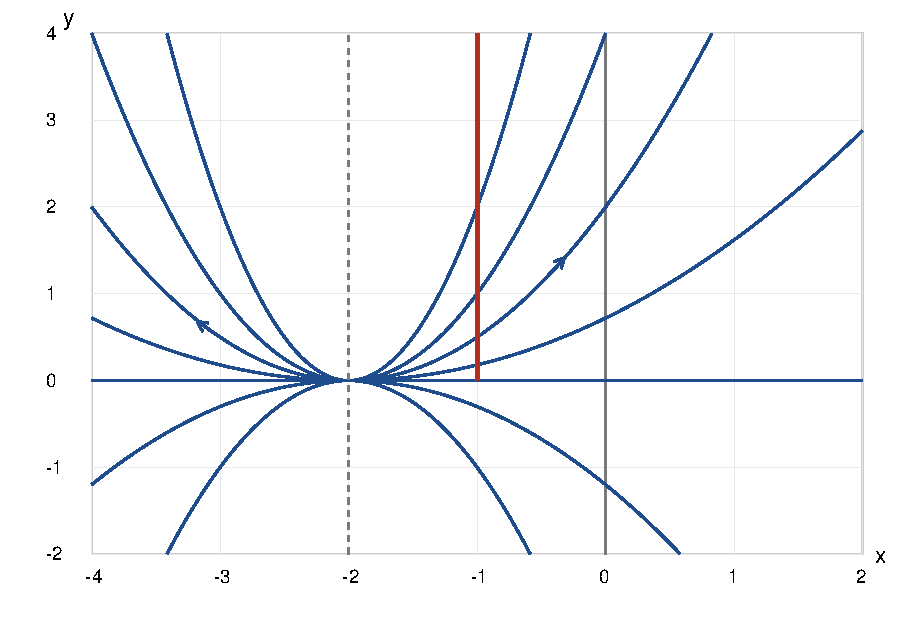
\includegraphics[width=.85\linewidth]{problem-1.pdf}
\end{center}
\emph{Sketch.} Blue curves are $y=C(x+2)^2$. The red half-line is the initial set $x=-1$, $y>0$. The dashed line is $x=-2$. The arrows indicate increasing characteristic time.
\end{samepage}

\step{Step 2: Write the required ODE using $x$ as parameter.}
On a characteristic $y=y(x)$,
\[
 \frac{\mathrm d}{\mathrm dx}u(x,y(x))
 =u_x+\frac{2y}{x+2}u_y
 =\frac{2u}{x+2}.
\]
Consequently
\[
 \frac{\mathrm d}{\mathrm dx}\left(\frac{u}{(x+2)^2}\right)=0.
\]
Thus $u/(x+2)^2$ is constant along each characteristic. This derivation also includes the identically zero solution, without dividing by $u$.

\step{Step 3: Apply the data and eliminate the parameters.}
Label the initial point by $s>0$:
\[
 X(s,0)=-1,\quad Y(s,0)=s,\quad U(s,0)=\sqrt{s}.
\]
Integrating the system gives
\[
 X+2=e^t,\qquad Y=se^{2t},\qquad U=\sqrt{s}\,e^{2t}.
\]
Since $e^t>0$, these characteristics remain in $x>-2$. Also $Y>0$. Conversely, every $(x,y)$ with $x>-2$, $y>0$ has the unique labels
\[
 t=\log(x+2),\qquad s=\frac{y}{(x+2)^2}>0.
\]
Therefore
\[
 u(x,y)=(x+2)^2\sqrt{\frac{y}{(x+2)^2}}
       =(x+2)\sqrt y,
\]
because $x+2>0$ on the domain in question.
\answer{u(x,y)=(x+2)\sqrt y,\qquad x>-2,\ y>0.}

\step{Step 4: Check transversality and verify.}
Here $(x_0',y_0')=(0,1)$ and $(a,b)=(1,2s)$ at the initial point, so $J_0=-1\ne0$. For the proposed solution,
\[
 u_x=\sqrt y,\qquad u_y=\frac{x+2}{2\sqrt y},
\]
and hence $(x+2)u_x+2yu_y=2(x+2)\sqrt y=2u$. At $x=-1$ its value is $\sqrt y$ as required.

The same expression is a smooth extension to the larger half-plane $y>0$. The data determine it uniquely only on $x>-2$, $y>0$: characteristics on the other side of $x=-2$ do not meet the initial set. No $C^1$ extension across $y=0$ near the initial line can preserve these data, since $\sqrt y$ has unbounded derivative at $0$.

\problem{Radial characteristics in the first quadrant}
\begin{question}
Consider $xu_x+yu_y=2u$ for $x>0$, $y>0$. Plot the characteristic curves and solve with (a) $u=1$ on $xy=1$; (b) $u=1$ on $x^2+y^2=1$. (c) Can general initial data be prescribed on $y=e^x$? Justify.
\end{question}
\step{Step 1: Solve the common characteristic equations.}
We have $X_t=X$, $Y_t=Y$, $U_t=2U$, giving
\[
 X=x_0e^t,\quad Y=y_0e^t,\quad U=u_0e^{2t}.
\]
Thus $Y/X=y_0/x_0$ is constant: the characteristics are rays from the origin. On each ray, scaling position by $\lambda>0$ scales $u$ by $\lambda^2$.
Equivalently, in the first quadrant the general form is
\[
 u(x,y)=x^2\Phi(y/x).
\]
To check this, put $m=y/x$ and compute
\[
 u_x=2x\Phi(m)-y\Phi'(m),\qquad u_y=x\Phi'(m).
\]
Then $xu_x+yu_y=2x^2\Phi(m)=2u$.

\begin{samepage}
\begin{center}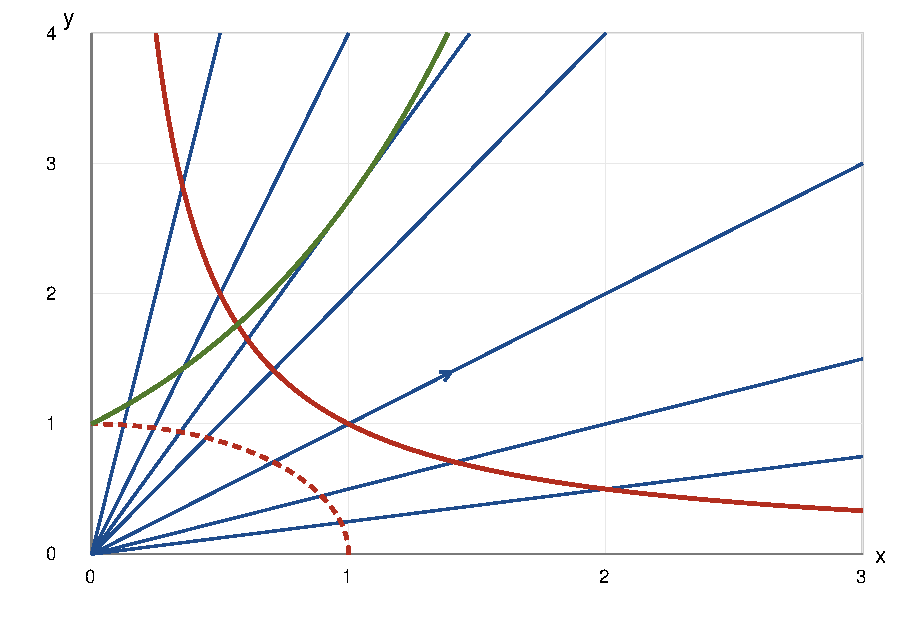
\includegraphics[width=.86\linewidth]{problem-2.pdf}\end{center}
\emph{Sketch.} Blue rays are characteristics. The solid red curve is $xy=1$, the dashed red arc is $x^2+y^2=1$, and the green curve is $y=e^x$. The latter is tangent to the ray $y=ex$ at $(1,e)$.
\end{samepage}

\subsection*{(a) Data on the hyperbola}
Write a point on the initial hyperbola as $(s,1/s)$, $s>0$. Since its initial value is $1$,
\[
 x=se^t,\qquad y=s^{-1}e^t,\qquad u=e^{2t}.
\]
Multiplying the equations for $x$ and $y$ gives $xy=e^{2t}$, so
\answer{u(x,y)=xy\quad(x>0,\ y>0).}
Every first-quadrant ray meets this hyperbola exactly once: $s=\sqrt{x/y}$ and $t=\frac12\log(xy)$. Hence the solution is unique throughout this quadrant. Transversality also follows from
\[
 J_0=\det\begin{pmatrix}1&s\\-s^{-2}&s^{-1}\end{pmatrix}=\frac2s\ne0.
\]
Directly, $u_x=y$, $u_y=x$, so $xu_x+yu_y=2xy$; on $xy=1$, $u=1$.

\subsection*{(b) Data on the circle}
Use the first-quadrant arc $(\cos s,\sin s)$ with $0<s<\pi/2$. Then
\[
 x=e^t\cos s,\qquad y=e^t\sin s,\qquad u=e^{2t}.
\]
Squaring and adding gives $x^2+y^2=e^{2t}$ and therefore
\answer{u(x,y)=x^2+y^2\quad(x>0,\ y>0).}
Each ray meets this arc exactly once, giving global uniqueness in the quadrant. The determinant is
\[
 J_0=(-\sin s)\sin s-(\cos s)\cos s=-1.
\]
Finally, $xu_x+yu_y=2x^2+2y^2=2u$, and $u=1$ on the unit circle.

\subsection*{(c) General data on the exponential curve}
Let $u(s,e^s)=g(s)$ for $s>0$. The determinant is
\[
 J_0=\det\begin{pmatrix}1&s\\e^s&e^s\end{pmatrix}=e^s(1-s).
\]
Thus arbitrary smooth data give a unique local solution near each initial point with $s\ne1$. At $s=1$, the initial curve is tangent to a characteristic, and compatibility must be checked.

The general form gives the necessary relation
\[
 g(s)=s^2\Phi\!\left(\frac{e^s}{s}\right).
\]
The slope function $m(s)=e^s/s$ satisfies
\[
 m'(s)=\frac{e^s(s-1)}{s^2}.
\]
It decreases on $(0,1)$, increases on $(1,\infty)$, and has minimum $e$. Consequently rays of slope $m>e$ meet the curve twice, the ray $m=e$ is tangent, and rays $0<m<e$ never meet it.

If two parameters $s_1\ne s_2$ have $e^{s_1}/s_1=e^{s_2}/s_2$, a solution on the entire quadrant must satisfy
\[
 \frac{g(s_1)}{s_1^2}=\frac{g(s_2)}{s_2^2}.
\]
Otherwise the two prescribed values on the same ray contradict the characteristic scaling law. At the tangency, differentiating $g(s)=u(s,e^s)$ gives
\[
 g'(1)=u_x(1,e)+eu_y(1,e)=2u(1,e)=2g(1).
\]
This first-derivative condition is necessary, but alone is not sufficient to guarantee the repeated-ray compatibility or smoothness of the induced function $\Phi$ at $m=e$.

For example, $g\equiv1$ violates $g'(1)=2g(1)$, so it gives no local $C^1$ solution at $(1,e)$. In contrast, $g(s)=se^s$ is compatible and is realized by $u=xy$. Even for compatible data, the slopes $0<m<e$ remain unprescribed, so a solution on the whole quadrant need not be unique. Problem 11(d) makes this last point explicit.

\problem{Four characteristic geometries}
\begin{question}
Sketch the characteristic curves and the initial curve, and solve:
\begin{enumerate}[label=(\alph*)]
\item $xu_x+yu_y=ku$, $x\in\R$, $y\ge\alpha>0$; $u(x,\alpha)=F(x)$, with $k,\alpha$ fixed and $F$ smooth.
\item $yu_x-xu_y=0$; $u(x,0)=x^2$.
\item $x^2u_x-y^2u_y=0$; $u(1,y)=F(y)$.
\item $yu_x+xu_y=0$; $u(0,y)=e^{-y^2}$.
\end{enumerate}
\end{question}
\subsection*{(a) Rays meeting a horizontal initial line}
\step{Step 1: Integrate the characteristic equations.}
Starting at $(s,\alpha,F(s))$, solve
\[
 X_t=X,\quad Y_t=Y,\quad U_t=kU.
\]
This gives $X=se^t$, $Y=\alpha e^t$, $U=F(s)e^{kt}$. Since $y\ge\alpha$, we use $t\ge0$. From the second equation,
\[
 e^t=y/\alpha,\qquad s=\alpha x/y.
\]
Substitution gives
\answer{u(x,y)=\left(\frac y\alpha\right)^k F\!\left(\frac{\alpha x}{y}\right),\quad y\ge\alpha.}
The real power is well defined even for nonintegral $k$ because $y/\alpha>0$.

\step{Step 2: Explain uniqueness and verify.}
The initial tangent is $(1,0)$, while the field is $(s,\alpha)$, so $J_0=\alpha\ne0$. Every point in the prescribed domain has exactly one $s$ and $t$ above. Thus the solution is unique there.
Put $A=(y/\alpha)^k$ and $\xi=\alpha x/y$. Since $\xi_x=\alpha/y$ and $\xi_y=-\xi/y$,
\[
 u_x=A F'(\xi)\frac\alpha y,\qquad
 u_y=\frac A y\bigl(kF(\xi)-\xi F'(\xi)\bigr).
\]
It follows that
\[
 xu_x+yu_y=A\xi F'(\xi)+A\bigl(kF(\xi)-\xi F'(\xi)\bigr)=ku.
\]
At $y=\alpha$, $A=1$ and $\xi=x$, yielding $u(x,\alpha)=F(x)$.
\begin{samepage}
\begin{center}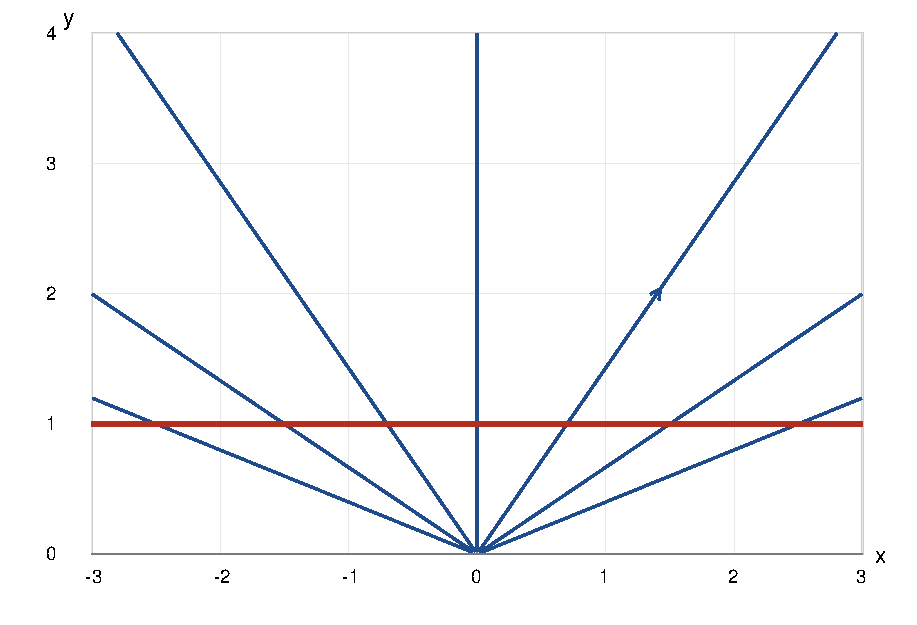
\includegraphics[width=.8\linewidth]{problem-3a.pdf}\end{center}
\emph{Sketch.} The figure uses $\alpha=1$ for illustration. The blue rays meet the red initial line once. The vertical ray $x=0$ is included.
\end{samepage}

\subsection*{(b) Circles meeting the horizontal axis}
\step{Step 1: Find the invariant.}
Here $X_t=Y$, $Y_t=-X$, $U_t=0$. Therefore
\[
 \frac{\mathrm d}{\mathrm dt}(X^2+Y^2)=2XY-2YX=0.
\]
Nonzero characteristics are circles centered at the origin, travelled clockwise. At the origin the vector field vanishes. As $U_t=0$, the value of $u$ is constant on each circle.

\step{Step 2: Use the values where the circles meet the data.}
A circle of radius $r>0$ meets $y=0$ at $(r,0)$ and $(-r,0)$. Both prescribed values are $r^2$, so the two intersections are compatible. Every point on that circle must have value $r^2$. At the origin the initial value is $0$. Hence
\answer{u(x,y)=x^2+y^2\quad\hbox{on }\R^2.}
This is the unique global classical solution. At $(s,0)$, $J_0=-s$, so the standard local theorem applies when $s\ne0$. Although it fails at $s=0$, the circle argument in any sufficiently small disk proves local uniqueness there as well.

\step{Step 3: Verify.}
The derivatives are $u_x=2x$, $u_y=2y$, and $yu_x-xu_y=2xy-2xy=0$. The trace at $y=0$ is $x^2$.
\begin{samepage}
\begin{center}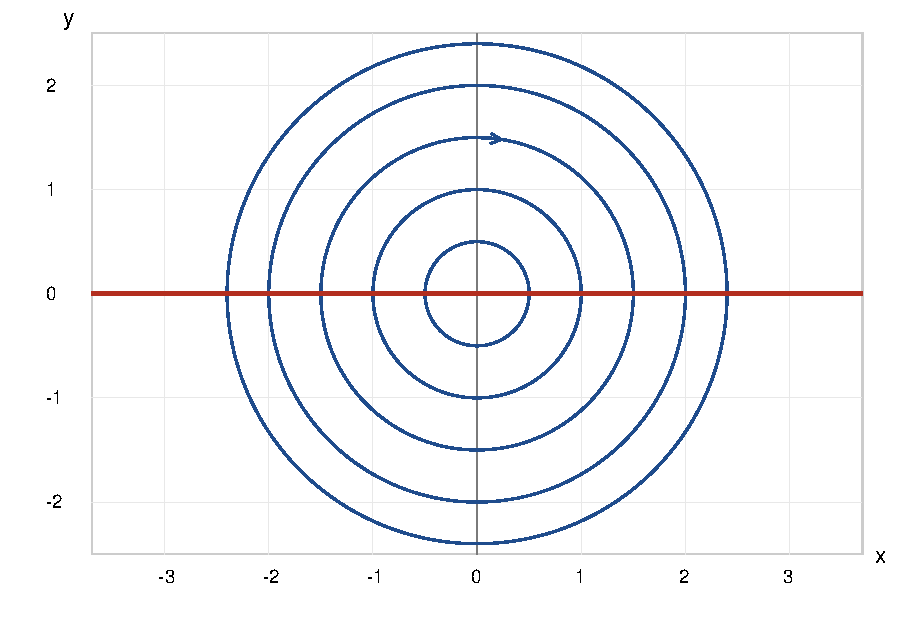
\includegraphics[width=.8\linewidth]{problem-3b.pdf}\end{center}
\emph{Sketch.} The blue circles meet the red initial axis twice; the two data values agree. The arrow indicates clockwise motion.
\end{samepage}

\subsection*{(c) Rational characteristic curves}
\step{Step 1: Integrate without losing the zero initial value.}
Use $(X,Y,U)(s,0)=(1,s,F(s))$. The equations are
\[
 X_t=X^2,\qquad Y_t=-Y^2,\qquad U_t=0.
\]
For $X$, $(1/X)_t=-1$, hence $X=1/(1-t)$. For $Y$, direct substitution verifies $Y=s/(1+st)$, including $s=0$. Thus
\[
 X=\frac1{1-t},\qquad Y=\frac{s}{1+st},\qquad U=F(s).
\]
The connected parameter interval containing $t=0$ must satisfy
\[
 1-t>0,\qquad 1+st>0.
\]
These conditions prevent crossing a finite-time pole of either ODE.

\step{Step 2: Recover the initial footpoint.}
From $x=1/(1-t)$, obtain $t=1-1/x$. The other equation yields
\[
 y=\frac{s}{1+s(1-1/x)}
 \quad\Longrightarrow\quad
 xy=s(x+y-xy).
\]
Define $D=x+y-xy$. We then have $s=xy/D$. Also $1+st=x/D$, so the characteristic domain is precisely
\[
 \Omega=\{(x,y):x>0,\ D=x+y-xy>0\}.
\]
Every point of $\Omega$ has a unique initial footpoint, and conversely the finite characteristic segments from $x=1$ lie in $\Omega$. Therefore
\answer{u(x,y)=F\!\left(\frac{xy}{x+y-xy}\right),\qquad (x,y)\in\Omega.}
In particular $y=0$ causes no difficulty: the formula gives $F(0)$.

\step{Step 3: Describe the curves and verify.}
Where $xy\ne0$,
\[
 \frac1x+\frac1y=1+\frac1s
\]
is constant. These are rational curves; the coordinate axes are invariant curves that division by $xy$ would omit. The data at $x=1$ have tangent $(0,1)$, so $J_0=-1\ne0$.

For $\xi=xy/D$, the quotient rule gives
\[
 \xi_x=\frac{y^2}{D^2},\qquad \xi_y=\frac{x^2}{D^2}.
\]
Hence
\[
 x^2u_x-y^2u_y=F'(\xi)\left(\frac{x^2y^2}{D^2}-\frac{y^2x^2}{D^2}\right)=0.
\]
At $x=1$, $D=1$ and $\xi=y$, proving the initial condition. No extension to all of $\R^2$ is asserted for arbitrary $F$: the initial-footpoint expression may become singular at $D=0$, and other characteristic regions are not determined by these data.
\begin{samepage}
\begin{center}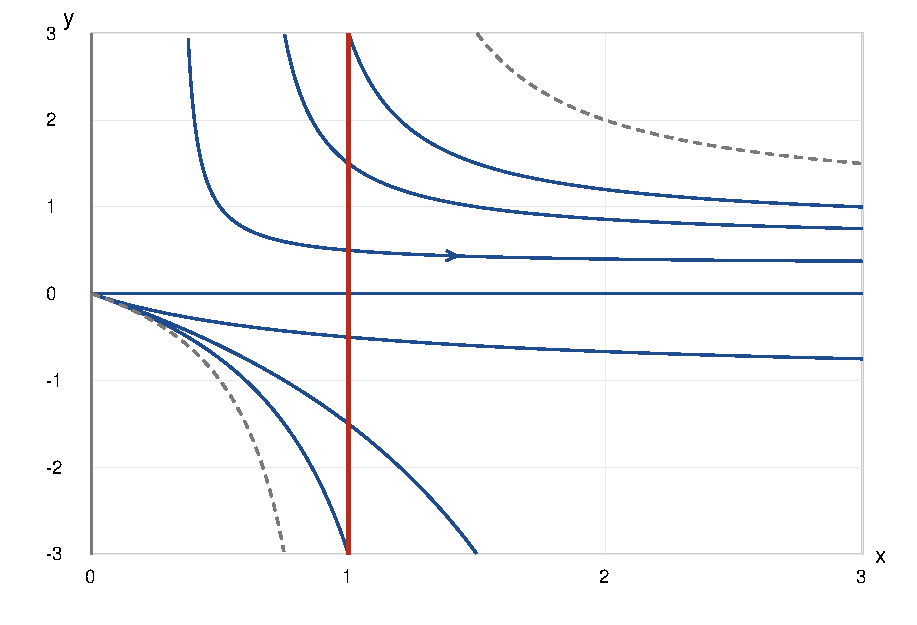
\includegraphics[width=.8\linewidth]{problem-3c.pdf}\end{center}
\emph{Sketch.} Blue curves are the segments reached from the red line $x=1$. The dashed curve $D=0$ bounds the determined region where it lies in the viewing window.
\end{samepage}

\subsection*{(d) Hyperbolas meeting the vertical axis}
\step{Step 1: Integrate the characteristic system.}
Starting at $(0,s,e^{-s^2})$, solve $X_t=Y$, $Y_t=X$, $U_t=0$. Since $X_{tt}=X$ and $X(0)=0$, $X_t(0)=s$,
\[
 X=s\sinh t,\qquad Y=s\cosh t,\qquad U=e^{-s^2}.
\]
Thus $Y^2-X^2=s^2$ and, for $s\ne0$, $|Y|>|X|$. Conversely any point with $|y|>|x|$ has
\[
 s=\operatorname{sgn}(y)\sqrt{y^2-x^2},\qquad
 t=\operatorname{artanh}(x/y).
\]
Consequently
\answer{u(x,y)=e^{x^2-y^2}\quad\hbox{on }|y|>|x|.}
The initial determinant is $J_0=-s$. Therefore the solution is locally unique near every nonzero point of the initial axis, and uniquely determined on the upper and lower open cones.

\step{Step 2: Give a global extension and verify it.}
The function $u_0=e^{x^2-y^2}$ is smooth on the whole plane. With $H=x^2-y^2$,
\[
 (y\partial_x+x\partial_y)H=2xy-2xy=0.
\]
The chain rule therefore gives $(y\partial_x+x\partial_y)e^H=0$. At $x=0$, its value is $e^{-y^2}$, so $u_0$ is a global solution.

\step{Step 3: Explain why that extension is not unique.}
The data do not intersect the hyperbolas in $|x|>|y|$. Define the smooth function
\[
 \psi(r)=\begin{cases}e^{-1/r},&r>0,\\0,&r\le0.\end{cases}
\]
Every derivative from the right at $r=0$ is $0$, since $e^{-1/r}$ tends to zero faster than any power of $r$. Thus this piecewise definition is $C^\infty$. For any constant $c$,
\[
 u_c=e^H+c\psi(H)
\]\nopagebreak
is a smooth global solution: $H$ is constant along characteristics, and $\psi(-y^2)=0$ on the initial axis. Different $c$ give different solutions arbitrarily close to the origin. Hence even \emph{smooth local uniqueness fails at the origin}, although existence holds. Continuity fixes the values $u=1$ on $y=\pm x$, but does not fix the values in the two horizontal cones.
\begin{samepage}
\begin{center}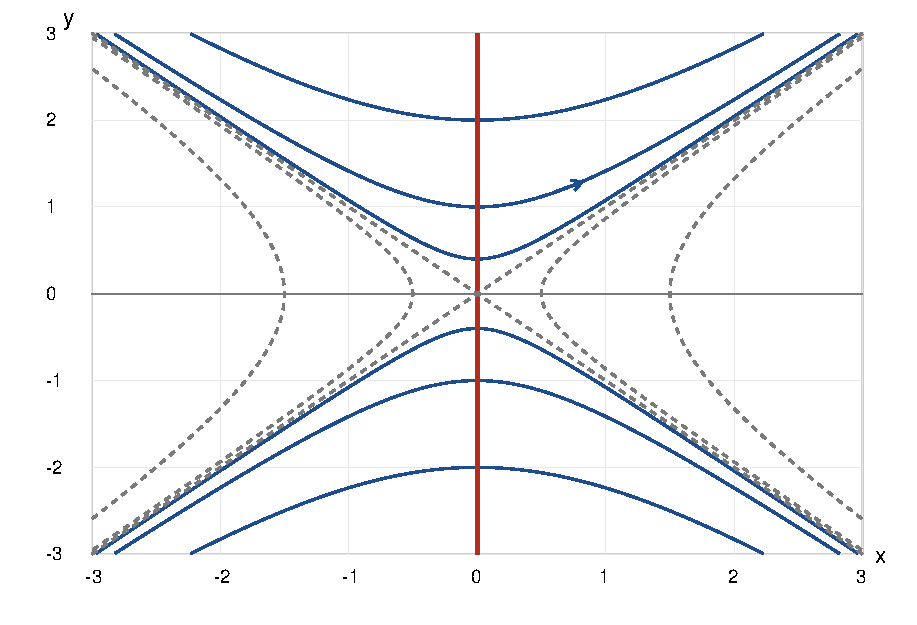
\includegraphics[width=.8\linewidth]{problem-3d.pdf}\end{center}
\emph{Sketch.} The blue hyperbolas meet the red initial axis. Gray dashed hyperbolas in the horizontal cones do not meet it. The diagonals are the characteristic boundaries $y=\pm x$.
\end{samepage}

\problem{Quasilinear equations and transversality}
\begin{question}
Solve the quasilinear problems and verify transversality:
\begin{enumerate}[label=(\alph*)]
\item $uu_x+u_y=0$, $u(x,0)=x$.
\item $uu_x+u_y=1$, $u(x,x)=x/2$, $x\in(0,1]$.
\end{enumerate}
\end{question}
\subsection*{(a) The homogeneous equation}
\step{Step 1: Integrate the characteristic equations.}
Here the speed in the $x$ direction is the unknown value $u$ itself. Use
\[
 X_t=U,\quad Y_t=1,\quad U_t=0,\qquad
 (X,Y,U)(s,0)=(s,0,s).
\]
The third equation gives $U=s$. The second gives $Y=t$. Substituting $U=s$ into the first and integrating gives $X=s+st=s(1+t)$.

\step{Step 2: Invert and identify the domain.}
The equations $y=t$, $x=s(1+y)$ give $s=x/(1+y)$ when $y\ne-1$. The connected characteristic domain containing the initial line is $y>-1$, so
\answer{u(x,y)=\frac{x}{1+y},\qquad x\in\R,\ y>-1.}
The initial determinant is $J_0=1$, because the tangent is $(1,0)$ and the characteristic vector is $(s,1)$. At later times,
\[
 \det\frac{\partial(X,Y)}{\partial(s,t)}
 =\det\begin{pmatrix}1+t&s\\0&1\end{pmatrix}=1+t=1+y.
\]
It first vanishes, going backwards from $y=0$, at $y=-1$.

\step{Step 3: Explain the obstruction at $y=-1$.}
Each characteristic is the line $x=s(1+y)$ and carries the value $u=s$. At $y=-1$, every such line reaches $(0,-1)$. Two different labels $s_1\ne s_2$ would require two different values at the same point. Therefore there is no continuous, and hence no classical, extension through that point. In particular, this IVP has no classical solution on the entire plane. The algebraic expression on $y<-1$ solves the PDE there, but is not a continuation through the breakdown.

\step{Step 4: Verify the formula.}
We have $u_x=1/(1+y)$ and $u_y=-x/(1+y)^2$. Thus
\[
 uu_x+u_y=\frac{x}{(1+y)^2}-\frac{x}{(1+y)^2}=0,
\]
and $u(x,0)=x$.

\subsection*{(b) A source term and a sloping initial curve}
\step{Step 1: Start at the prescribed spatial and solution values.}
For $0<s\le1$ the data are $(X,Y,U)(s,0)=(s,s,s/2)$. Therefore
\[
 X_t=U,\qquad Y_t=1,\qquad U_t=1.
\]
Integrate $U_t=1$ and $Y_t=1$ first:
\[
 U=\frac{s}{2}+t,\qquad Y=s+t.
\]
Now integrate $X_t=s/2+t$ with $X(s,0)=s$:
\[
 X=s+\frac{s}{2}t+\frac{t^2}{2}.
\]
The projected characteristics are parabolas.

\step{Step 2: Check the initial determinant.}
The initial tangent is $(1,1)$ and the characteristic direction there is $(s/2,1)$. Thus
\[
 J_0=1-\frac{s}{2}>0\qquad(0<s\le1).
\]
The data are noncharacteristic. This verifies the requested transversality condition.

\step{Step 3: Eliminate $s$ and $t$ carefully.}
From $y=s+t$ obtain $t=y-s$. Substitute this into $x$:
\begin{align*}
 x&=s+\frac{s}{2}(y-s)+\frac12(y-s)^2\\
  &=s+\frac{sy}{2}-\frac{s^2}{2}
       +\frac{y^2}{2}-ys+\frac{s^2}{2}\\
  &=\frac{y^2}{2}+s\left(1-\frac y2\right).
\end{align*}
The two $s^2/2$ terms cancel. Therefore, when $y\ne2$,
\[
 s=\frac{2x-y^2}{2-y},\qquad U=y-\frac{s}{2}.
\]
It follows that
\answer{u(x,y)=y-\frac{2x-y^2}{2(2-y)}
              =\frac{4y-y^2-2x}{2(2-y)}.}
The part determined by the stated initial labels, before breakdown, is
\[
 y<2,\qquad 0<\frac{2x-y^2}{2-y}\le1.
\]
On the interior $0<s<1$ this is an open characteristic region. The edge $s=1$ is included as a trace. The displayed expression also gives a smooth extension to the whole half-plane $y<2$, but values outside the region with $0<s\le1$ are not prescribed by the original data.

\step{Step 4: Check the later Jacobian and explain the breakdown.}
Differentiate the parametric formula:
\[
 X_s=1+t/2,\quad X_t=s/2+t,\quad Y_s=1,\quad Y_t=1.
\]
Consequently
\[
 J=1+\frac t2-\left(\frac s2+t\right)
  =1-\frac{s+t}{2}=1-\frac y2.
\]
The first degeneracy along forward characteristics is at $y=2$. Putting $t=2-s$ in the parametric formulas gives
\[
 (X,Y)=(2,2),\qquad U=2-\frac{s}{2}.
\]
Thus all these characteristics meet at $(2,2)$ with incompatible values. No continuous solution satisfying all the data can include that point.

\step{Step 5: Verify the PDE and the chosen branch of the data.}
Write $d=2-y$ and $R=2x-y^2$. Then $u=y-R/(2d)$ and
\[
 u_x=-\frac1d,\qquad
 u_y=1+\frac yd-\frac{R}{2d^2}.
\]
Hence
\[
 uu_x+u_y=-\frac yd+\frac{R}{2d^2}
                 +1+\frac yd-\frac{R}{2d^2}=1.
\]
At $(x,y)=(s,s)$, $R=s(2-s)$, so $u=s-s/2=s/2$.

\problem{Existence and uniqueness for a constant transport field}
\begin{question}
For $u_x+u_y=0$ on $\R^2$, discuss existence and uniqueness under
\[
 \text{(a) }u(x,-x)=x,\qquad
 \text{(b) }u(x,x)=x,\qquad
 \text{(c) }u(x,x)=1.
\]
\end{question}
\step{Step 1: Find the full family of solutions.}
The characteristic equations $X_t=1$, $Y_t=1$, $U_t=0$ show that $X-Y$ is constant and that $u$ is constant along the lines $x-y=c$. Therefore every classical solution on the entire plane has the form
\[
 u(x,y)=\Phi(x-y),\qquad \Phi\in C^1(\R).
\]
Indeed, each line meets $y=0$ once, so $\Phi(r)=u(r,0)$ determines its value. Conversely, $u_x=\Phi'(x-y)$ and $u_y=-\Phi'(x-y)$ verify the PDE for every such $\Phi$.

\subsection*{(a) Data on the line $y=-x$}
Parameterize the initial line by $(s,-s)$. Then
\[
 \Phi(2s)=s\quad\hbox{for every }s\in\R.
\]
Since $2s$ ranges over all real numbers, this forces $\Phi(r)=r/2$ for every $r$. Thus
\answer{u(x,y)=\frac{x-y}{2}\quad\hbox{is the unique global solution}.}
The determinant is $1\cdot1-(-1)\cdot1=2\ne0$, and every characteristic meets the data once. Directly $u(s,-s)=s$.

\subsection*{(b) Nonconstant data on a characteristic line}
The line $y=x$ is a single characteristic, so $u$ must be constant on it. But the prescribed value $u(s,s)=s$ is not constant. Equivalently, the formula above would require $\Phi(0)=s$ for every $s$, which is impossible.

There is no local classical solution near any point of this initial line that satisfies the data on a nontrivial segment. Another way to see the contradiction is to differentiate the trace:
\[
 \frac{\mathrm d}{\mathrm ds}u(s,s)=u_x(s,s)+u_y(s,s)=0,
\]
whereas the derivative of the prescribed trace $s$ is $1$.

\subsection*{(c) Constant data on a characteristic line}
This time the compatibility requirement is simply $\Phi(0)=1$. There are infinitely many choices:
\[
 u(x,y)=\Phi(x-y),\qquad\Phi\in C^1(\R),\quad\Phi(0)=1.
\]
For example $u_1=1$ and $u_2=1+x-y$ are distinct smooth global solutions with the same initial values. They also differ in every neighborhood of the initial line, so both global and local uniqueness fail. For (b) and (c), the determinant is $1\cdot1-1\cdot1=0$; these two cases illustrate respectively incompatible and compatible characteristic data.

\problem{The diagonal-segment IVP, including its endpoints}
\begin{question}
Solve $uu_x+u_y=1$ with initial conditions $x=s$, $y=s$, $u=s/2$, where $0\le s\le1$.
\end{question}
This repeats Problem 4(b) with the additional endpoint $s=0$. We give the construction again so the answer can be read independently.

\step{Step 1: Solve the characteristic system.}
Use $t=0$ on the initial segment. The system and its solution are
\[
 X_t=U,\quad Y_t=1,\quad U_t=1,
\]
\[
 X=s+\frac{st}{2}+\frac{t^2}{2},\qquad
 Y=s+t,\qquad U=\frac{s}{2}+t.
\]
These satisfy the initial conditions immediately on setting $t=0$.

\step{Step 2: Recover $s$ and $t$.}
The second equation gives $t=y-s$. Substitution into the first simplifies to
\[
 x=\frac{y^2}{2}+\frac{s(2-y)}2.
\]
For $y\ne2$,
\[
 s=\frac{2x-y^2}{2-y},\qquad t=y-\frac{2x-y^2}{2-y}.
\]
Since $u=s/2+t=y-s/2$, the solution is
\answer{u(x,y)=\frac{4y-y^2-2x}{2(2-y)}.}

\step{Step 3: Describe exactly the region supplied by the segment.}
On the side $y<2$ containing the initial segment, $2-y$ is positive. Thus $0\le s\le1$ is equivalent to
\[
 0\le2x-y^2\le2-y.
\]
The determined region, with its two characteristic edges, is therefore
\[
 y<2,\qquad \frac{y^2}{2}\le x\le\frac{y^2+2-y}{2}.
\]
The left edge is the characteristic from $s=0$, the right edge the characteristic from $s=1$. Their separation at a fixed height is $(2-y)/2$, which tends to zero as $y\uparrow2$. The open interior is a classical solution domain; the formula is smooth across either edge if a larger domain is desired.

\step{Step 4: Check noncharacteristic data and the point of failure.}
Initially $J_0=1-s/2\ge1/2$, including both endpoints. Later the Jacobian is $1-y/2$. At $y=2$, all characteristics arrive at $(2,2)$, but the transported values range from $2$ at $s=0$ to $3/2$ at $s=1$. A single-valued continuous solution cannot have all these values at one point. Hence no global classical solution on $\R^2$ exists.

\step{Step 5: Verify the explicit answer.}
As in Problem 4(b), setting $d=2-y$, $R=2x-y^2$ gives $u=y-R/(2d)$, $u_x=-1/d$ and $u_y=1+y/d-R/(2d^2)$. These identities yield $uu_x+u_y=1$. At $(s,s)$, $R=s(2-s)$ and hence $u=s/2$, including $s=0,1$.

\textbf{Endpoint qualification.} Nonzero $J_0$ guarantees local uniqueness from data on an open initial arc. At an endpoint of a finite initial segment, the stated data determine the solution only on the corresponding one-sided characteristic region. To prescribe the solution on a full open neighborhood of an endpoint, one may extend $s/2$ smoothly beyond $[0,1]$. The formula above uses that natural extension. Different smooth extensions beyond an endpoint can give different solutions on its unprescribed side. This qualification also applies to the endpoint $s=1$ in Problem 4(b).

\problem{Two characteristic solutions of the eikonal equation}
\begin{question}
For $p^2+q^2=1$, where $p=u_x$, $q=u_y$, and $u=0$ on $x+y=1$, find the two solutions by the method of characteristics.
\end{question}
\step{Step 1: Determine the possible initial gradients.}
Parameterize the initial line by $(x_0,y_0)=(s,1-s)$. The derivative of its constant trace is zero, so
\[
 p\,x_0'+q\,y_0'=p-q=0.
\]
Combining $p=q$ with $p^2+q^2=1$ gives
\[
 p=q=\frac{\varepsilon}{\sqrt2},\qquad \varepsilon\in\{+1,-1\}.
\]
These are the two possible normal gradient directions. For a $C^1$ solution the sign cannot switch along the connected initial line: $p$ is continuous there and can take only these two nonzero values.

\step{Step 2: Write and integrate the fully nonlinear characteristic system.}
Set $H=p^2+q^2-1$. Since $H$ is independent of $x,y,u$,
\[
 X_t=2p,\quad Y_t=2q,\quad p_t=0,\quad q_t=0,
\]
\[
 U_t=pH_p+qH_q=2(p^2+q^2)=2.
\]
With the initial data, this gives
\[
 X=s+\varepsilon\sqrt2\,t,\qquad
 Y=1-s+\varepsilon\sqrt2\,t,\qquad U=2t.
\]
The projected characteristics are the straight lines normal to $x+y=1$.

\step{Step 3: Eliminate the parameters.}
Adding the two coordinate equations gives $x+y-1=2\varepsilon\sqrt2\,t$. Therefore $2t=\varepsilon(x+y-1)/\sqrt2$, and
\answer{u_+(x,y)=\frac{x+y-1}{\sqrt2},\qquad
 u_-(x,y)=-\frac{x+y-1}{\sqrt2}.}
For either choice, every point of $\R^2$ lies on exactly one characteristic from the initial line. Its label is $s=(x-y+1)/2$.

\step{Step 4: Check transversality and verify.}
The determinant for either gradient branch is
\[
 \det\begin{pmatrix}1&\varepsilon\sqrt2\\-1&\varepsilon\sqrt2\end{pmatrix}
 =2\varepsilon\sqrt2\ne0.
\]
Hence each branch gives a locally unique smooth characteristic solution, but the prescribed \emph{values} alone admit two branches. For the displayed solutions, $u_x=u_y=\varepsilon/\sqrt2$, so $u_x^2+u_y^2=1$. Both vanish on $x+y=1$.

The phrase ``two solutions'' here refers to the two classical characteristic branches. The expression $|x+y-1|/\sqrt2$ is not a further classical solution across the initial line, because its gradient jumps there.

\problem{A global obstruction: construction still to be resolved}
\begin{question}
Find a smooth $a:\R^2\to\R$ such that
\[
 a(x,y)u_x+u_y=0
\]
has no solution on the entire plane for any nonconstant initial value prescribed on $\{y=0\}$.
\end{question}
\textbf{Status of this problem.} A coefficient satisfying the full quantifier ``for any nonconstant initial value'' has not been established in this draft. The calculations below are verified, but do not solve that construction problem. They are included to prevent a false nonexistence proof from entering a student solution sheet. No claim is being made that the original statement is impossible or that it is a confirmed misprint.

\step{Step 1: Explain what the characteristic method actually proves.}
If $u(x,0)=g(x)$, then characteristics starting at $s$ satisfy
\[
 \frac{\mathrm dX}{\mathrm dy}=a(X,y),\qquad X(0)=s,
 \qquad u(X(y),y)=g(s).
\]
Because the initial tangent is $(1,0)$ and the field is $(a(s,0),1)$, the determinant is always $1$. Thus smooth data have local solutions. The problem asks for a specifically \emph{global} obstruction, valid for every nonconstant $g$.

The failure of an individual characteristic to exist for all $y$ does not imply that $u$ fails to exist on the entire plane. A characteristic may escape to spatial infinity without making $u$ singular at any finite point.

\step{Step 2: Test the tempting candidate $a=x^2$.}
The ODE $X_y=X^2$, $X(0)=s$ gives
\[
 X(y)=\frac{s}{1-sy},\qquad
 s=\frac{x}{1+xy}.
\]
On the region reached from $y=0$, namely $1+xy>0$, the initial-value formula is
\[
 u(x,y)=g\!\left(\frac{x}{1+xy}\right).
\]
For some choices of $g$, this formula does prevent a global extension. For example, if $g(s)=s$, its values on $(1,y)$ become unbounded as $y\downarrow-1$ from above. Therefore the IVP with these particular data has no continuous global solution.

However, this does not establish nonexistence for \emph{every} nonconstant $g$.

\step{Step 3: Give a smooth nonconstant-data counterexample to that candidate.}
Define
\[
 v(x,y)=\begin{cases}
 \exp\!\left[-\left(y+\dfrac1x\right)^2\right],&x\ne0,\\[3pt]
 0,&x=0.
 \end{cases}
\]
For $x\ne0$, put $I=y+1/x$. Since $I_x=-1/x^2$ and $I_y=1$,
\[
 x^2v_x+v_y=-2I e^{-I^2}(x^2I_x+I_y)=0.
\]
The piecewise definition is smooth across $x=0$. To see why, restrict $y$ to a bounded interval $|y|\le M$. For sufficiently small $|x|$,
\[
 \left|y+\frac1x\right|\ge\frac1{2|x|}.
\]
Every derivative of the expression for $x\ne0$ is a finite sum of a polynomial in $y,1/x$ times $e^{-(y+1/x)^2}$. Its absolute value is therefore bounded by a constant times $|x|^{-N}e^{-1/(4x^2)}$, which tends to $0$ for every fixed $N$. All derivatives extend by zero at $x=0$. The PDE holds there too, since $v_y(0,y)=0$.

Its initial trace is
\[
 g(x)=\begin{cases}e^{-1/x^2},&x\ne0,\\0,&x=0,\end{cases}
\]
which is smooth and nonconstant. Thus $a=x^2$ does \emph{not} answer the original question.

\step{A related problem that can be solved completely.}
If the requested statement were instead to exhibit \emph{some} smooth nonconstant data with no global solution, $a=x^2$ with $g(x)=x$ would answer it, by Step 2.

Another related statement concerns the \emph{quasilinear} equation
\[
 uu_x+u_y=0,\qquad u(x,0)=g(x).
\]
For this equation, every nonconstant $C^1$ datum prevents a classical solution on the entire plane. Indeed, choose $s_1\ne s_2$ with $g(s_1)\ne g(s_2)$. Its two characteristics are
\[
 x=s_i+y g(s_i),\qquad u=g(s_i),\qquad i=1,2.
\]
They intersect at the finite height
\[
 y_*=-\frac{s_1-s_2}{g(s_1)-g(s_2)}.
\]
At their intersection a single-valued solution would have to equal both $g(s_1)$ and $g(s_2)$, a contradiction. This proves the related assertion, but the coefficient here is $u$, not a preassigned smooth function $a(x,y)$, so it is not a solution of the original construction problem.

\problem{Radial characteristics in three dimensions}
\begin{question}
Consider $xu_x+yu_y+zu_z=3u$ in $\R^3$.
\begin{enumerate}[label=(\alph*)]
\item Solve with $u(x,y,1)=x^2+y^2$.
\item Is it possible to find a unique solution if initial data are prescribed on $z=1+x^2+y^2$?
\end{enumerate}
\end{question}
\subsection*{(a) Data on the plane $z=1$}
\step{Step 1: Integrate the four characteristic equations.}
Label the initial point by $(s,r,1)$, with initial value $s^2+r^2$. The system is
\[
 X_t=X,\quad Y_t=Y,\quad Z_t=Z,\quad U_t=3U.
\]
Consequently
\[
 X=se^t,\quad Y=re^t,\quad Z=e^t,\quad
 U=(s^2+r^2)e^{3t}.
\]
As in the two-dimensional radial examples, the projected characteristics are rays from the origin; now $u$ scales with degree $3$.

\step{Step 2: Eliminate the parameters.}
Since $Z=e^t>0$, the data determine the solution on $z>0$. Given a point in that half-space,
\[
 e^t=z,\quad s=x/z,\quad r=y/z.
\]
Substituting in $U$ gives
\[
 u=\left(\frac{x^2}{z^2}+\frac{y^2}{z^2}\right)z^3=z(x^2+y^2).
\]
Thus
\answer{u(x,y,z)=z(x^2+y^2)\quad\hbox{on }z>0.}
The normal to the initial plane is $(0,0,1)$ and its dot product with the field $(s,r,1)$ is $1$. The surface is noncharacteristic, and every ray in $z>0$ meets it once. Therefore the solution is unique on $z>0$.

\step{Step 3: Verify the formula and discuss extension.}
For $u_0=z(x^2+y^2)$,
\[
 u_{0x}=2xz,\quad u_{0y}=2yz,\quad u_{0z}=x^2+y^2.
\]
Hence
\[
 xu_{0x}+yu_{0y}+zu_{0z}
 =2x^2z+2y^2z+z(x^2+y^2)=3u_0.
\]
At $z=1$, $u_0=x^2+y^2$. This polynomial supplies a smooth solution on all of $\R^3$.

In the $C^1$ class the global extension is not unique. Define
\[
 h(z)=\begin{cases}z^3,&z<0,\\0,&z\ge0.\end{cases}
\]
The function $h$ is $C^2$ and satisfies $zh'(z)=3h(z)$, including at $z=0$. Therefore $u_0+c h(z)$, $c\in\R$, gives distinct global $C^1$ (indeed $C^2$) solutions with the same data. No characteristic from $z=1$ reaches $z<0$.

If one requires a global $C^3$ solution, the answer is unique. To justify this carefully, write $P=(x,y,z)$. The PDE implies $u(\lambda P)=\lambda^3u(P)$ for $\lambda>0$, by differentiating $\lambda^{-3}u(\lambda P)$. Also $u(0)=0$ by the PDE at zero. The third-order Taylor expansion has the form
\[
 u(\lambda P)=\lambda L(P)+\lambda^2Q(P)+\lambda^3C(P)+o(\lambda^3),
\]
where $L,Q,C$ are the homogeneous Taylor terms of degrees $1,2,3$. Comparing with $\lambda^3u(P)$ and first dividing by $\lambda$ gives $L(P)=0$ as $\lambda\downarrow0$. Dividing the remaining identity by $\lambda^2$ gives $Q(P)=0$. Finally division by $\lambda^3$ gives $u(P)=C(P)$. Thus $u$ is a homogeneous cubic polynomial. Since this polynomial agrees with $z(x^2+y^2)$ on the open set $z>0$, it agrees everywhere. In particular the global smooth solution is unique.

\subsection*{(b) Data on the paraboloid}
\step{Step 1: Compute the normal component of the characteristic field.}
Write the initial surface as
\[
 S=\{G=0\},\qquad G(x,y,z)=z-1-x^2-y^2.
\]
Its normal is $\nabla G=(-2x,-2y,1)$. On $S$,
\[
 (x,y,z)\cdot\nabla G=-2x^2-2y^2+z=1-x^2-y^2.
\]
Thus the surface is noncharacteristic where $x^2+y^2\ne1$, and characteristic along the circle
\[
 x^2+y^2=1,\qquad z=2.
\]
Arbitrary smooth data determine a unique local solution near each noncharacteristic point. The same conclusion cannot be asserted at the tangency circle.

\step{Step 2: Derive the necessary compatibility at tangency.}
Suppose the trace is $u(x,y,1+x^2+y^2)=g(x,y)$. Along the surface,
\[
 g_x=u_x+2xu_z,\qquad g_y=u_y+2yu_z.
\]
At $x^2+y^2=1$, we therefore obtain
\[
 xg_x+yg_y=xu_x+yu_y+2u_z
          =xu_x+yu_y+zu_z=3g.
\]
Thus the necessary condition is
\answer{xg_x+yg_y=3g\quad\hbox{on }x^2+y^2=1.}
For example, $g\equiv1$ violates this identity ($0\ne3$), so it admits no local $C^1$ solution at the tangency circle. Conversely, some data do admit a solution: the polynomial from (a) has trace $g=(1+x^2+y^2)(x^2+y^2)$ on the paraboloid.

\step{Step 3: Explain the additional global obstruction.}
Let $P=(x,y,1+r^2)$, $r^2=x^2+y^2>0$. Another point $\lambda P$ on the same ray belongs to the paraboloid precisely if
\[
 \lambda(1+r^2)=1+\lambda^2r^2.
\]
Factoring gives
\[
 (\lambda-1)(\lambda r^2-1)=0.
\]
Thus, unless $r=1$, the ray meets the surface twice: at $P$ and at $P/r^2$. Since $u$ scales cubically along rays, any global solution must satisfy
\[
 g\!\left(\frac{x}{r^2},\frac{y}{r^2}\right)=\frac{g(x,y)}{r^6}.
\]
Generic data do not satisfy this repeated-intersection condition. Moreover, rays outside the upward cone $z\ge2\sqrt{x^2+y^2}$ do not meet the surface. Indeed, a ray through $(x,y,z)$ meets it only if $\lambda z=1+\lambda^2(x^2+y^2)$ has a positive solution. For $x^2+y^2>0$ this requires $z>0$ and discriminant $z^2-4(x^2+y^2)\ge0$; the positive vertical ray also meets the surface.

Therefore there is no general existence-and-uniqueness assertion for data on the entire paraboloid: local uniqueness holds off the tangency circle; at that circle compatibility is essential; and global solvability and uniqueness require further analysis of the data and the solution class.

\problem{Initial gradients for two fully nonlinear equations}
\begin{question}
Consider the IVPs
\[
 \text{A: }u=u_x^2-3u_y^2,\qquad u(x,0)=x^2,\quad x>0,
\]
\[
 \text{B: }u=u_xu_y,\qquad u(x,0)=x^2,\quad x>0.
\]
(a) Discuss existence and uniqueness of both IVPs. (b) Solve any one. We solve both to make the difference in uniqueness explicit.
\end{question}
\subsection*{A: Two admissible initial gradients}
\step{Step 1: Use the differentiated data and the PDE on the initial line.}
At $(s,0)$ with $s>0$, the trace gives
\[
 U_0=s^2,\qquad p_0=\frac{\mathrm d}{\mathrm ds}(s^2)=2s.
\]
Inserting these into $p_0^2-3q_0^2=U_0$ gives
\[
 4s^2-3q_0^2=s^2\quad\Longrightarrow\quad q_0^2=s^2.
\]
Hence $q_0=\varepsilon s$ with $\varepsilon=+1$ or $-1$. The initial data do not choose between these two normal derivatives. The sign is fixed on a connected initial interval for any $C^1$ solution, because $q_0/s$ is continuous and takes values only in $\{-1,+1\}$.

\step{Step 2: Check the determinant for each branch.}
Let $H=p^2-3q^2-u$. Then $H_p=2p$, $H_q=-6q$. For the initial curve $(s,0)$,
\[
 J_0=H_q=-6\varepsilon s\ne0.
\]
Thus each choice of initial gradient gives a locally unique smooth solution by the noncharacteristic characteristic construction. There are two choices, so the IVP with values alone is not locally unique.

\step{Step 3: Integrate the characteristic equations.}
Since $H_x=H_y=0$ and $H_u=-1$, the full system becomes
\[
 X_t=2p,\quad Y_t=-6q,\quad p_t=p,\quad q_t=q,
\]
\[
 U_t=2p^2-6q^2=2U.
\]
The last equality uses $H=0$ along the characteristics; the integrated formulas below verify that relation directly. With the initial values,
\[
 p=2se^t,\quad q=\varepsilon se^t,\quad U=s^2e^{2t},
\]
\[
 X=s+4s(e^t-1)=s(4e^t-3),\qquad
 Y=-6\varepsilon s(e^t-1).
\]

\step{Step 4: Eliminate the parameters and verify.}
The useful combinations are
\[
 x+\frac{\varepsilon y}{2}=se^t,\qquad
 x+\frac{2\varepsilon y}{3}=s.
\]
Therefore
\answer{u_{\varepsilon}(x,y)=\left(x+\frac{\varepsilon y}{2}\right)^2,
 \qquad\varepsilon=\pm1.}
For $L=x+\varepsilon y/2$, the derivatives are $u_x=2L$, $u_y=\varepsilon L$. Hence
\[
 u_x^2-3u_y^2=4L^2-3L^2=L^2=u.
\]
At $y=0$, both give $x^2$, and their normal derivatives are $\pm x$, as calculated initially.

The characteristic region from $s>0$ for each branch is
\[
 x+\frac{2\varepsilon y}{3}>0,\qquad
 x+\frac{\varepsilon y}{2}>0,
\]
because these quantities are $s$ and $se^t$, respectively. The polynomial expressions nevertheless extend smoothly to the entire plane. In particular, two distinct global smooth solutions exist.

\subsection*{B: One admissible initial gradient}
\step{Step 1: Determine the initial gradient.}
Again $U_0=s^2$ and $p_0=2s$. The PDE gives $p_0q_0=s^2$, so
\[
 q_0=\frac{s^2}{2s}=\frac{s}{2}.
\]
The restriction $s>0$ is essential for this division. Unlike A, there is exactly one possible initial normal derivative.

\step{Step 2: Check noncharacteristic data.}
For $H=pq-u$, we have $H_p=q$, $H_q=p$, $H_u=-1$. Hence $J_0=H_q=p_0=2s\ne0$. There is a unique local smooth solution near each point of the stated initial half-line. This is the local uniqueness conclusion for the IVP, not a claim that the data determine the entire plane.

\step{Step 3: Integrate the characteristic equations.}
They are
\[
 X_t=q,\quad Y_t=p,\quad p_t=p,\quad q_t=q,\quad U_t=2pq=2U.
\]
Solving with $(X,Y,U,p,q)(s,0)=(s,0,s^2,2s,s/2)$ yields
\[
 p=2se^t,\quad q=\frac s2 e^t,\quad U=s^2e^{2t},
\]
\[
 X=s+\frac s2(e^t-1)=\frac s2(1+e^t),\qquad
 Y=2s(e^t-1).
\]
From these equations,
\[
 x-\frac y4=s,\qquad x+\frac y4=se^t.
\]
Consequently
\answer{u(x,y)=\left(x+\frac y4\right)^2.}

\step{Step 4: Verify and distinguish local from global uniqueness.}
With $L=x+y/4$, $u_x=2L$ and $u_y=L/2$. Thus $u_xu_y=L^2=u$, and at $y=0$, $u=x^2$. The characteristic domain determined by the half-line is
\[
 x-\frac y4>0,\qquad x+\frac y4>0,
\]
i.e. $x>|y|/4$. The polynomial provides a smooth global extension.

If global uniqueness is asked in the $C^1$ class, it does not follow from the local theorem. For an explicit alternative, put $L_+=\max\{L,0\}$ and define
\[
 \widetilde u(x,y)=(L_+)^2.
\]
For $L>0$ it equals the polynomial solution; for $L<0$ it is zero, which also satisfies $u=u_xu_y$. On $L=0$, its value and both first derivatives are zero, so it is a global $C^1$ solution. Its trace on $y=0$, $x>0$ is $x^2$. It is different from the polynomial where $L<0$, but agrees with it on the determined characteristic domain. It is not $C^2$ along $L=0$.

Thus the intended local comparison is: A has two characteristic branches and is not unique; B has one noncharacteristic branch and is locally unique. Both have global smooth solutions, while global $C^1$ uniqueness fails for both.

\problem{Local and global uniqueness on the whole plane}
\begin{question}
For $xu_x+yu_y=2u$ on $\R^2$, discuss both global and local existence and uniqueness with the following data. If uniqueness fails, give an alternative solution on $\R^2$.
\begin{enumerate}[label=(\alph*)]
\item $u=1$ on $xy=1$, $x>0$.
\item $u=1$ on $y=1$.
\item $u=1$ on $x^2+y^2=1$.
\item $u(x,e^x)=xe^x$ for every $x\in\R$.
\end{enumerate}
\end{question}
\step{A common fact: the PDE is a homogeneity equation.}
Let $P=(x,y)\ne(0,0)$. For $\lambda>0$, the chain rule gives
\begin{align*}
 \frac{\mathrm d}{\mathrm d\lambda}\bigl[\lambda^{-2}u(\lambda x,\lambda y)\bigr]
 &=-2\lambda^{-3}u(\lambda x,\lambda y)
   +\lambda^{-2}\bigl[xu_x(\lambda P)+yu_y(\lambda P)\bigr]\\
 &=\lambda^{-3}\bigl[-2u(\lambda P)
     +(\lambda x)u_x(\lambda P)+(\lambda y)u_y(\lambda P)\bigr]=0.
\end{align*}
Therefore any global classical solution satisfies
\[
 u(\lambda x,\lambda y)=\lambda^2u(x,y),\qquad\lambda>0.
\]
Such a function is called \emph{positively homogeneous of degree two}. At the origin the PDE gives $0=2u(0,0)$, so $u(0,0)=0$.

In polar coordinates the general form away from the origin is
\[
 u(r\cos\theta,r\sin\theta)=r^2 A(\theta),\qquad r>0.
\]
Here $A$ is a $2\pi$-periodic $C^1$ function. Every such $A$ gives a global $C^1$ solution by setting $u(0,0)=0$: $|u|=O(r^2)$ proves differentiability at the origin with derivative zero, and the polar differentiation formulas give $|\nabla u|=O(r)$, proving continuity of the first derivatives. This makes it possible to alter values on rays not meeting the data.

For simple explicit alternatives, define $r_-:=\max\{-r,0\}$. The function $r_-^2$ is $C^1$: it equals $r^2$ for $r<0$, zero for $r\ge0$, and both one-sided first derivatives at zero are zero. It also satisfies
\[
 r\frac{\mathrm d}{\mathrm dr}(r_-^2)=2r_-^2
\]
on all of $\R$.

\subsection*{(a) Data on the positive branch of a hyperbola}
\step{Step 1: Determine the solution on rays that meet the data.}
As in Problem 2(a), the rays meeting $(s,1/s)$, $s>0$, fill precisely the first quadrant. At $(x,y)$ in that quadrant, the characteristic calculation gives $u=xy$. The initial determinant is $2/s\ne0$, so there is a unique local solution near each initial point.

\step{Step 2: Exhibit distinct global classical extensions.}
The polynomial $u_0=xy$ is a global smooth solution. For any real constant $c$,
\answer{u_c(x,y)=xy+c\,x_-^2}
is a global $C^1$ solution. Indeed, the Euler operator $x\partial_x+y\partial_y$ sends $xy$ to $2xy$ and $x_-^2$ to $2x_-^2$. Hence it sends $u_c$ to $2u_c$. On the prescribed hyperbola $x>0$, the added term is zero and $xy=1$. Choosing $c=0$ and $c=1$ gives two distinct solutions. Thus global $C^1$ existence holds and uniqueness fails, although local uniqueness holds at every point of the initial curve.

\subsection*{(b) Data on the horizontal line $y=1$}
\step{Step 1: Follow rays from the initial line.}
Starting at $(s,1)$ with $U_0=1$, the characteristic equations give
\[
 x=se^t,\qquad y=e^t,\qquad u=e^{2t}.
\]
Consequently $u=y^2$ throughout $y>0$. Every point there is reached once, with $s=x/y$. The initial determinant is $1$, so the solution is locally unique at every initial point.

\step{Step 2: Give global alternatives.}
For any $c\in\R$,
\answer{u_c(x,y)=y^2+c\,y_-^2}
is global and $C^1$, satisfies the PDE by the homogeneity identity above, and has value $1$ at $y=1$. Different $c$ give different values in $y<0$. Thus there is no global $C^1$ uniqueness. The data determine the upper half-plane and, by continuity, $u(x,0)=0$, but not the lower half-plane.

\subsection*{(c) Data on the whole unit circle}
\step{Step 1: Use the fact that every ray is prescribed.}
Every nonzero point can be uniquely written $(x,y)=r(\cos\theta,\sin\theta)$, with $r=\sqrt{x^2+y^2}>0$. The initial value at the unit point is $1$. By degree-two scaling,
\[
 u(x,y)=r^2\cdot1=x^2+y^2.
\]
At the origin the PDE forces $u(0,0)=0$, exactly the polynomial value. Hence
\answer{u(x,y)=x^2+y^2\quad\hbox{is the unique global classical solution}.}
The initial determinant is $-1$, as in Problem 2(b), giving local uniqueness at every point of the circle. Substitution gives $xu_x+yu_y=2x^2+2y^2=2u$, and the initial trace is $1$. There is no distinct global alternative with the same data.

\subsection*{(d) Compatible data on the exponential curve}
\step{Step 1: Verify existence before discussing uniqueness.}
The polynomial $u_0=xy$ solves the PDE and has $u_0(s,e^s)=se^s$. Thus existence holds, including at the tangency point $(1,e)$.

The initial determinant is $e^s(1-s)$. It is nonzero for every $s\ne1$, including $s=0$ and negative $s$. The local solution is therefore unique near each of those initial points. At $s=1$, the necessary compatibility condition from Problem 2(c) is satisfied: for $g(s)=se^s$,
\[
 g'(1)=(1+1)e=2e=2g(1).
\]

\step{Step 2: Identify which rays are fixed by the data.}
A point reached by scaling $(s,e^s)$ has
\[
 (x,y)=(\lambda s,\lambda e^s),\qquad
 u=\lambda^2se^s=xy.
\]
All such points have $y>0$. For $s<0$, the ratio $x/y=se^{-s}$ increases strictly from $-\infty$ to $0$ as $s$ increases to $0$, since its derivative is $e^{-s}(1-s)>0$. These initial points cover all rays in the second quadrant, and $s=0$ supplies the positive vertical ray.

For $s>0$, the slope $y/x=e^s/s$ ranges over $[e,\infty)$, with two initial intersections for slopes greater than $e$. The values are compatible at these two intersections because the quantity $u/x^2$ prescribed there is $e^s/s$, exactly the ray slope.

Thus the data determine $u=xy$ on
\[
 \{x\le0,\ y>0\}\ \cup\ \{x>0,\ y\ge ex\}.
\]
They do not prescribe the first-quadrant rays $0<y<ex$, nor the rays in the lower half-plane.

\step{Step 3: Give explicit global $C^1$ alternatives.}
For every $c\in\R$,
\answer{u_c(x,y)=xy+c\,y_-^2}
is a global $C^1$ solution with the same trace, because $e^s>0$ makes the added term vanish on the entire initial curve. Hence global classical uniqueness fails.

\step{Step 4: Prove local nonuniqueness at the tangency point.}
The preceding alternatives differ only in the lower half-plane, so they do not by themselves prove local nonuniqueness near $(1,e)$. A separate construction is needed.

Use the flat function $\psi$ from Problem 3(d), and, in a neighborhood where $x>0$, define
\[
 v_c(x,y)=xy+c\,x^2\psi\!\left(e-\frac yx\right).
\]
Every expression $x^2\Phi(y/x)$ solves the radial PDE; the added term has this form, so $v_c$ solves it. It is smooth for $x>0$, including across $y=ex$, because $\psi$ is smooth and flat at zero.

On the initial curve with $s>0$, $e^s/s\ge e$, so $\psi(e-e^s/s)=0$. Thus all $v_c$ have the prescribed data near $(1,e)$. But every open neighborhood of $(1,e)$ contains points with $0<y<ex$, where the added term is nonzero if $c\ne0$. Hence local uniqueness at $(1,e)$ fails even among smooth local solutions.

This local alteration can also be made into a global $C^1$ alternative. Choose $0<m_0<m_1<e$ and a smooth cutoff $\chi$ equal to zero for $m\le m_0$ and one for $m\ge m_1$. One explicit choice, using the same $\psi$, is
\[
 \chi(m)=\frac{\psi(m-m_0)}{\psi(m-m_0)+\psi(m_1-m)}.
\]
Its denominator is positive for every real $m$, because $m_0<m_1$ prevents both arguments from being nonpositive. Set
\[
 w(x,y)=\begin{cases}
 x^2\chi(y/x)\psi(e-y/x),&x>0,\\0,&x\le0.
 \end{cases}
\]
It vanishes unless $m_0<y/x<e$, so it is zero near every nonzero point of the vertical axis. Away from the origin it is smooth. It is homogeneous of degree two, and its smooth angular factor has bounded derivative, so $w$ is $C^1$ at the origin by the general argument at the start of this problem. Thus $xy+cw$ gives global $C^1$ solutions that also demonstrate the local freedom at the tangency.

\subsection*{Why global $C^2$ or smooth solutions have a different answer}
\step{Step 1: Prove that global $C^2$ solutions must be quadratic forms.}
Suppose $u\in C^2(\R^2)$ solves the PDE. We already know $u(0)=0$ and $u(\lambda P)=\lambda^2u(P)$. Differentiability at zero gives
\[
 \nabla u(0)\cdot P
 =\lim_{\lambda\downarrow0}\frac{u(\lambda P)-u(0)}{\lambda}
 =\lim_{\lambda\downarrow0}\lambda u(P)=0.
\]
Since this holds for every $P$, $\nabla u(0)=0$. Taylor's theorem now gives
\[
 u(\lambda P)=\frac{\lambda^2}{2}P^T D^2u(0)P+o(\lambda^2).
\]
Divide by $\lambda^2$, use homogeneity on the left, and let $\lambda\downarrow0$. The result is
\[
 u(P)=\frac12P^TD^2u(0)P.
\]
Thus $u(x,y)=Ax^2+Bxy+Cy^2$ everywhere. This rigidity comes from regularity at the origin; away from the origin a smooth homogeneous function need not be a polynomial.

\step{Step 2: Determine the coefficients for each set of data.}
\begin{enumerate}[label=(\alph*)]
\item On $(s,1/s)$ with $s>0$, the condition is $As^2+B+C/s^2=1$. Multiplying by $s^2$ produces the polynomial identity $As^4+(B-1)s^2+C=0$ for all $s>0$, so $A=C=0$, $B=1$. Hence $u=xy$.
\item On $y=1$, $Ax^2+Bx+C=1$ for every $x$, so $A=B=0$, $C=1$. Hence $u=y^2$.
\item At $(1,0)$ and $(0,1)$ the data give $A=C=1$. At $(1/\sqrt2,1/\sqrt2)$ they give $1+B/2=1$, so $B=0$. Hence $u=x^2+y^2$.
\item In $Ax^2+Bxe^x+Ce^{2x}=xe^x$, put $x=0$ to obtain $C=0$. For $x\ne0$, divide by $x$ to obtain $Ax+(B-1)e^x=0$. Dividing again by $x$ and letting $x\to-\infty$ yields $A=0$; then $B=1$. Hence $u=xy$.
\end{enumerate}
Therefore all four problems have unique \emph{global $C^2$}, and thus unique global smooth, solutions. The $C^1$ alternatives above are not counterexamples to this conclusion, since they are not $C^2$ on the entire plane. Smooth local nonuniqueness at $(1,e)$ in (d) still holds: a local neighborhood there need not include the origin.

\subsection*{Comparison table}
\begin{center}
\small
\begin{tabular}{@{}p{.08\linewidth}p{.27\linewidth}p{.30\linewidth}p{.23\linewidth}@{}}
\toprule
Data & Global $C^1$ solutions & Local uniqueness & Global $C^2$ solution\\
\midrule
(a) & Exist; not unique & Yes, at every point & Unique: $xy$\\[5pt]
(b) & Exist; not unique & Yes, at every point & Unique: $y^2$\\[5pt]
(c) & Unique: $x^2+y^2$ & Yes, at every point & Unique: $x^2+y^2$\\[5pt]
(d) & Exist; not unique & Yes except $(1,e)$; fails there & Unique: $xy$\\
\bottomrule
\end{tabular}
\end{center}

\clearpage
\section*{Reference and final checks for the reader}
\addcontentsline{toc}{section}{Reference and final checks for the reader}
The course reference is A. K. Nandakumaran and P. S. Datti,
\emph{Partial Differential Equations: Classical Theory with a Modern Touch},
Cambridge University Press, 2020. The bibliographic details are confirmed on
\href{https://math.iisc.ac.in/~nands/publications.html}{A. K. Nandakumaran's publications page}.
These solutions use the characteristic-ODE approach; no textbook solution or theorem numbering is assumed.

The questions have been transcribed from the supplied \texttt{problems.pdf}, retaining its numbering, data, and parameter restrictions. The derivations and checks are supplied in these notes. Problem 8 remains explicitly unresolved; the related results in that section are not substitutes for its original quantifier.

When checking a first-order Cauchy problem, keep the following four questions separate:
\begin{enumerate}
\item \textbf{Does the candidate solve the PDE?} Compute its derivatives and substitute.
\item \textbf{Does it have the required initial trace?} Substitute the initial curve or surface, including any endpoints or exceptional points.
\item \textbf{Where is it determined by the data?} Trace the characteristics back to the initial set and check the inverse map, signs, and possible singularities.
\item \textbf{In which regularity class is it unique?} A $C^1$ extension and a $C^2$ or smooth extension can have different uniqueness properties, especially at the origin of a radial field.
\end{enumerate}
\end{document}
